%%%% CAPÍTULO 4 - RESULTADOS E DISCUSSÃO

\chapter{Resultados e Discussão}\label{cap:resultados}

Este capítulo apresenta e discute os resultados obtidos sobre o conjunto de
4.180 partidas da \textit{Premier League} disputadas entre as temporadas
2015/16 e 2025/26. A Seção~\ref{sec:res-magnitude} quantifica a magnitude da
vantagem do mandante. A Seção~\ref{sec:res-faixa} examina a heterogeneidade
dessa vantagem entre equipes de diferentes faixas de classificação. As
Seções~\ref{sec:res-temporal} e~\ref{sec:res-publico} tratam, respectivamente,
da evolução temporal do fenômeno e do papel do público. As
Seções~\ref{sec:res-modelo} e~\ref{sec:res-preditivo} apresentam os resultados
da modelagem estatística e da modelagem preditiva, e a
Seção~\ref{sec:resultados-estadios} traz um estudo de caso sobre mudanças de
sede.

\section{Magnitude da Vantagem do Mandante}\label{sec:res-magnitude}

No recorte estudado, 44,33\% das partidas terminaram com vitória do mandante,
contra 31,99\% de vitórias do visitante e 23,68\% de empates. A
Tabela~\ref{tab:testes} reúne os testes de hipótese aplicados.

\begin{table}[htb]
  \centering
  \caption{Testes de hipótese sobre a vantagem do mandante.}
  \label{tab:testes}
  \resizebox{\textwidth}{!}{% Gerado por scripts/gerar_tabelas_latex.py --- não editar à mão.
\begin{tabular}{lrrccr}
  \toprule
  Teste & $n$ & Estimativa & IC 95\% & $p$ & Efeito \\
  \midrule
  Binomial (vitórias do mandante entre jogos decididos) & 3190 & 0,5809 & [0,564; 0,598] & $<10^{-19}$ & 1,386 \\
  Qui-quadrado (simetria casa/fora) & 4180 & 0,1234 & --- & $<10^{-19}$ & --- \\
  Teste $t$ pareado (diferença de pontos) & 4180 & 0,3703 & [0,292; 0,449] & $<10^{-19}$ & 0,143 \\
  Diferencial casa--fora: \textit{Big Six} vs.\ demais & 28 & 0,0514 & [$-$0,069; 0,172] & 0,351 & 0,465 \\
  Vantagem do mandante em 2019/20: com vs.\ sem público & 380 & $-$0,0190 & [$-$0,637; 0,599] & 0,952 & $-$0,007 \\
  \bottomrule
\end{tabular}
}
  \fonte{Autoria própria (2026)}
\end{table}

O teste binomial condicionado aos jogos decididos indica que o mandante vence
58,09\% deles, com intervalo de confiança de 95\% entre 56,35\% e 59,81\%. A
razão de chances correspondente é de 1,386, isto é, as chances de vitória do
mandante são aproximadamente 39\% maiores do que as do visitante. O teste
pareado sobre a diferença de pontos estima uma vantagem média de 0,37 ponto por
partida, com intervalo entre 0,29 e 0,45.

A significância estatística desses resultados é inequívoca. Cabe, entretanto,
atenção à magnitude: o $d$ de Cohen associado à diferença de pontos é de 0,143,
valor classificado como efeito pequeno segundo as faixas convencionais
de~\citeonline{Cohen1988}. Com uma amostra de 4.180 partidas, p-valores
reduzidos são esperados mesmo para diferenças modestas, e a interpretação
adequada do fenômeno exige considerar as duas informações conjuntamente. O Fator
Casa, no recorte analisado, é um efeito \textbf{consistente e sistemático, porém
de magnitude moderada}.

\subsection{Volume ou Eficiência?}\label{sec:res-conversao}

Uma questão correlata é se a vantagem do mandante decorre de maior eficiência na
finalização ou de maior volume de oportunidades criadas. A
Tabela~\ref{tab:conversao} apresenta a taxa de conversão de finalizações no alvo
em gols, calculada como a razão entre os totais do período.

\begin{table}[htb]
  \centering
  \caption{Taxa de conversão de finalizações no alvo em gols.}
  \label{tab:conversao}
  \small
  % Gerado por scripts/gerar_tabelas_latex.py --- não editar à mão.
\begin{tabular}{lrrrc}
  \toprule
  Mando & Gols & Chutes no alvo & Taxa & IC 95\% \\
  \midrule
  Mandante & 6477 & 19878 & 0,3258 & [0,3193; 0,3323] \\
  Visitante & 5322 & 16764 & 0,3175 & [0,3104; 0,3244] \\
  \bottomrule
\end{tabular}

  \fonte{Autoria própria (2026)}
\end{table}

As taxas são praticamente equivalentes: 32,58\% para mandantes e 31,75\% para
visitantes, com intervalos de confiança que quase se sobrepõem. Em contrapartida,
conforme apresentado na Seção~\ref{sec:res-temporal}, os mandantes produzem
sistematicamente mais finalizações no alvo e mais escanteios por partida. A
evidência, portanto, aponta que \textbf{o Fator Casa manifesta-se como volume de
oportunidades, e não como superioridade técnica na finalização de cada jogada
isolada}.

\section{Fator Casa por Faixa de Classificação}\label{sec:res-faixa}

Uma hipótese intuitiva sustenta que equipes de maior qualidade técnica
dependeriam menos do mando de campo, por serem capazes de impor seu jogo também
como visitantes. A Tabela~\ref{tab:faixa} e a Figura~\ref{fig:faixa} examinam
essa hipótese segmentando as equipes pela posição final em cada temporada.

\begin{table}[htb]
  \centering
  \caption{Vantagem do mandante por faixa de posição final.}
  \label{tab:faixa}
  \small
  % Gerado por scripts/gerar_tabelas_latex.py --- não editar à mão.
\begin{tabular}{lrrrrrrr}
  \toprule
  Faixa & Jogos & Pts casa & Pts fora & $\Delta$ pts & $\Delta$ gols & $\Delta$ chutes alvo & $\Delta$ escant. \\
  \midrule
  G6 (1-6) & 1254 & 2,180 & 1,730 & +0,450 & +0,430 & +1,096 & +1,190 \\
  Meio (7-14) & 1672 & 1,504 & 1,154 & +0,349 & +0,221 & +0,624 & +0,881 \\
  Z6 (15-20) & 1254 & 1,037 & 0,719 & +0,319 & +0,197 & +0,555 & +0,917 \\
  \bottomrule
\end{tabular}

  \fonte{Autoria própria (2026)}
\end{table}

\begin{figure}[htb]
  \centering
  \caption{Vantagem do mandante por faixa de posição final.}
  \label{fig:faixa}
  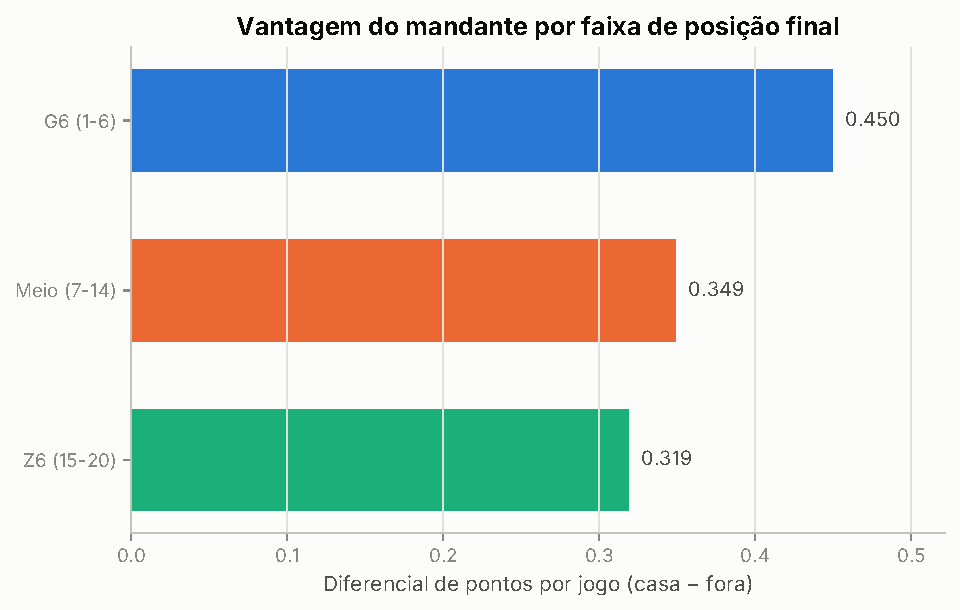
\includegraphics[width=0.75\textwidth]{./figuras/fator_casa_por_faixa.pdf}
  \fonte{Autoria própria (2026)}
\end{figure}

O resultado contraria a hipótese intuitiva. O gradiente é monotônico e aponta na
direção oposta: equipes que terminam entre as seis primeiras colocadas obtêm
vantagem de 0,450 ponto por partida ao jogar em casa, contra 0,349 das equipes
intermediárias e 0,319 das seis últimas. O mesmo ordenamento aparece em gols,
finalizações no alvo e escanteios, o que reduz a possibilidade de o achado ser
artefato de uma métrica específica.

A interpretação desse resultado deve considerar um efeito de teto. As equipes do
grupo G6 já conquistam, em média, 1,730 ponto por partida como visitantes,
restando-lhes apenas 1,270 ponto de margem até o máximo de três. As equipes do
Z6 conquistam 0,719 ponto fora e dispõem de 2,281 pontos de margem. Dispondo de
menos espaço para crescer, as equipes de maior qualidade ainda assim crescem
mais ao atuar em seus domínios. Normalizando o ganho pela margem disponível,
conforme a coluna de ganho relativo da Tabela~\ref{tab:clubes}, a diferença
entre os grupos torna-se ainda mais acentuada.

Esse achado tem implicação direta sobre a forma de operacionalizar o conceito de
qualidade técnica. A etapa anterior desta pesquisa comparava um grupo fixo de
seis clubes, convencionalmente denominado \textit{Big Six}, com os demais. Essa
operacionalização é problemática por duas razões: o grupo não é homogêneo ao
longo de um recorte de onze temporadas, e a comparação entre apenas dois grupos
descarta a informação ordinal da classificação. Quando a comparação é refeita
pela média do diferencial por clube, o grupo fixo apresenta 0,418 ponto contra
0,366 dos demais, diferença não significativa (Tabela~\ref{tab:testes},
$p = 0{,}351$), com intervalo de confiança compatível tanto com vantagem quanto
com desvantagem. A segmentação por posição final, por acompanhar a variação de
desempenho ao longo do tempo, revela a estrutura que a segmentação fixa não
captura.

\subsection{Variação entre Clubes}\label{sec:res-clubes}

A Tabela~\ref{tab:clubes} apresenta os clubes com maior diferencial no recorte,
restrita àqueles com pelo menos três temporadas disputadas.

\begin{table}[htb]
  \centering
  \caption{Clubes com maior diferencial casa--fora (mínimo de três temporadas).}
  \label{tab:clubes}
  \resizebox{\textwidth}{!}{% Gerado por scripts/gerar_tabelas_latex.py --- não editar à mão.
\begin{tabular}{lrrcrrrr}
  \toprule
  Clube & Jogos casa & Temp. & \textit{Big Six} & Pts casa & Pts fora & $\Delta$ pts & Ganho rel. \\
  \midrule
  Swansea & 57 & 3 & Não & 1,368 & 0,754 & +0,614 & 0,273 \\
  Arsenal & 209 & 11 & Sim & 2,201 & 1,612 & +0,589 & 0,424 \\
  Newcastle & 190 & 10 & Não & 1,626 & 1,058 & +0,568 & 0,293 \\
  Liverpool & 209 & 11 & Sim & 2,297 & 1,823 & +0,474 & 0,402 \\
  Sheffield United & 57 & 3 & Não & 1,035 & 0,596 & +0,439 & 0,182 \\
  Sunderland & 57 & 3 & Não & 1,246 & 0,807 & +0,439 & 0,200 \\
  Aston Villa & 152 & 8 & Não & 1,572 & 1,138 & +0,434 & 0,233 \\
  Man United & 209 & 11 & Sim & 1,952 & 1,531 & +0,421 & 0,287 \\
  Tottenham & 209 & 11 & Sim & 1,885 & 1,469 & +0,416 & 0,272 \\
  Brentford & 95 & 5 & Não & 1,537 & 1,126 & +0,411 & 0,219 \\
  \bottomrule
\end{tabular}
}
  \fonte{Autoria própria (2026)}
\end{table}

A restrição de amostra é necessária. Clubes que disputaram uma única temporada
no recorte acumulam apenas 19 partidas como mandantes, contra 209 dos clubes
presentes em todas as temporadas, e ocupam posições extremas do ranqueamento por
efeito da variabilidade amostral, e não por característica real de desempenho.

Entre os clubes com amostra suficiente, o diferencial varia de 0,614 ponto por
partida, no extremo superior, a 0,120 no inferior. A Figura~\ref{fig:dispersao}
posiciona cada clube segundo seu desempenho nas duas condições de mando: a
quase totalidade situa-se acima da linha de identidade, o que confirma que o
fenômeno afeta praticamente todos os competidores, ainda que em intensidades
distintas.

\begin{figure}[htb]
  \centering
  \caption{Desempenho das equipes como mandantes e como visitantes.}
  \label{fig:dispersao}
  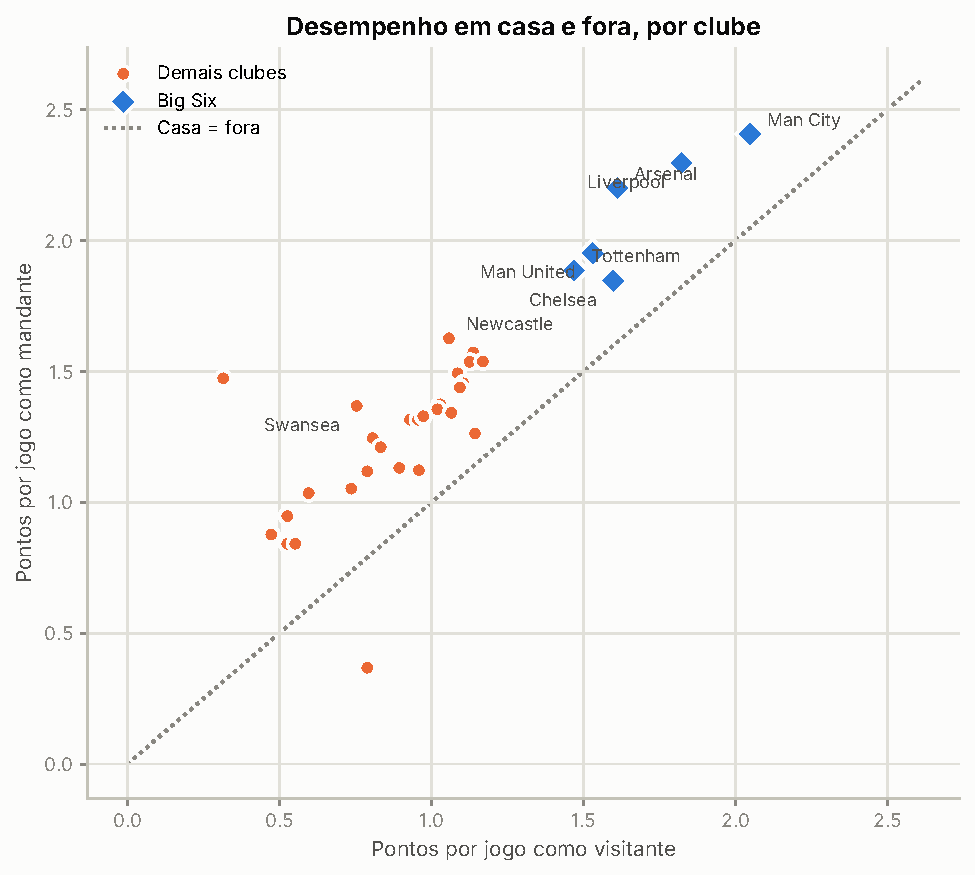
\includegraphics[width=0.72\textwidth]{./figuras/dispersao_casa_fora.pdf}
  \fonte{Autoria própria (2026)}
\end{figure}

\section{Evolução Temporal}\label{sec:res-temporal}

A Tabela~\ref{tab:evolucao} apresenta a evolução do diferencial de desempenho ao
longo das onze temporadas, incluindo métricas de volume ofensivo e disciplinares.

\begin{table}[htb]
  \centering
  \caption{Evolução temporal do diferencial entre mandantes e visitantes.}
  \label{tab:evolucao}
  \small
  % Gerado por scripts/gerar_tabelas_latex.py --- não editar à mão.
\begin{tabular}{lrrrrr}
  \toprule
  Temporada & $\Delta$ pts & Média móvel (3) & $\Delta$ chutes alvo & $\Delta$ escant. & $\Delta$ amarelos \\
  \midrule
  15/16 & +0,324 & --- & +0,747 & +1,061 & $-$0,208 \\
  16/17 & +0,616 & --- & +0,958 & +0,945 & $-$0,142 \\
  17/18 & +0,513 & +0,484 & +0,863 & +1,197 & $-$0,087 \\
  18/19 & +0,418 & +0,516 & +0,850 & +1,153 & $-$0,158 \\
  19/20 & +0,442 & +0,458 & +0,561 & +0,842 & $-$0,179 \\
  20/21 & $-$0,071 & +0,263 & +0,461 & +0,926 & $-$0,024 \\
  21/22 & +0,268 & +0,213 & +0,537 & +0,782 & $-$0,092 \\
  22/23 & +0,592 & +0,263 & +1,013 & +1,166 & $-$0,245 \\
  23/24 & +0,411 & +0,424 & +1,005 & +1,411 & $-$0,353 \\
  24/25 & +0,182 & +0,395 & +0,568 & +0,555 & $-$0,239 \\
  25/26 & +0,379 & +0,324 & +0,632 & +0,792 & $-$0,416 \\
  \bottomrule
\end{tabular}

  \fonte{Autoria própria (2026)}
\end{table}

O diferencial em pontos oscila de forma expressiva entre temporadas, de um
mínimo de $-0{,}071$ em 2020/21 a um máximo de $+0{,}616$ em 2016/17. A média
móvel de três temporadas situa-se entre 0,32 e 0,42 nas temporadas mais
recentes, contra valores entre 0,46 e 0,52 no início do período, padrão
compatível com uma redução moderada. As Figuras~\ref{fig:evolucao}
e~\ref{fig:diferencial} apresentam, respectivamente, as séries de pontos de
mandantes e visitantes e o diferencial entre elas.

\begin{figure}[htb]
  \centering
  \caption{Média de pontos por jogo de mandantes e visitantes, por temporada.}
  \label{fig:evolucao}
  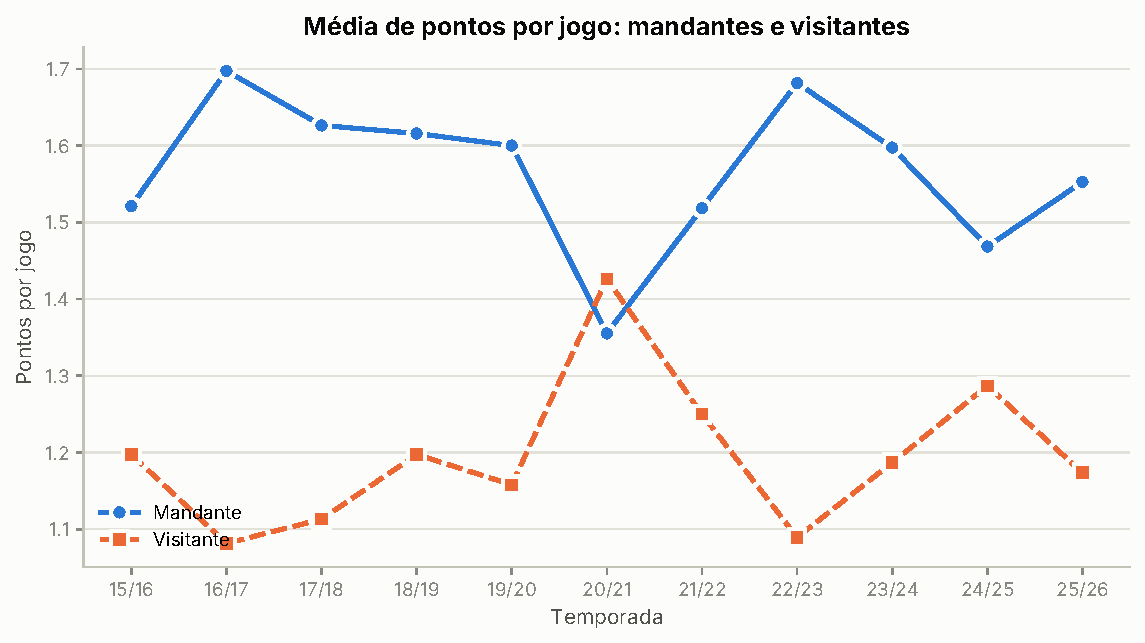
\includegraphics[width=0.9\textwidth]{./figuras/evolucao_pontos.pdf}
  \fonte{Autoria própria (2026)}
\end{figure}

\begin{figure}[htb]
  \centering
  \caption{Diferencial de pontos por jogo entre mandante e visitante.}
  \label{fig:diferencial}
  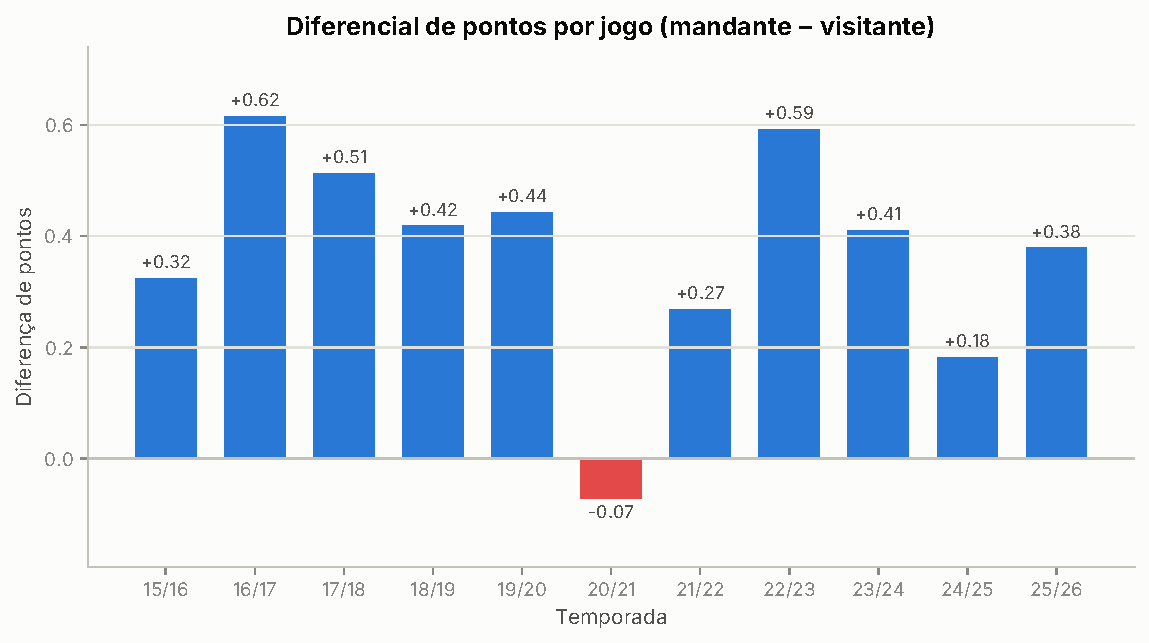
\includegraphics[width=0.9\textwidth]{./figuras/diferencial_por_temporada.pdf}
  \fonte{Autoria própria (2026)}
\end{figure}

As métricas de volume ofensivo acompanham o diferencial de pontos ao longo de
todo o período: os mandantes produzem, conforme a temporada, entre 0,46 e 1,01
finalização no alvo a mais e entre 0,56 e 1,41 escanteio a mais por partida. A
Figura~\ref{fig:volume} apresenta essa evolução.

\begin{figure}[htb]
  \centering
  \caption{Evolução das finalizações no alvo e dos escanteios por mando.}
  \label{fig:volume}
  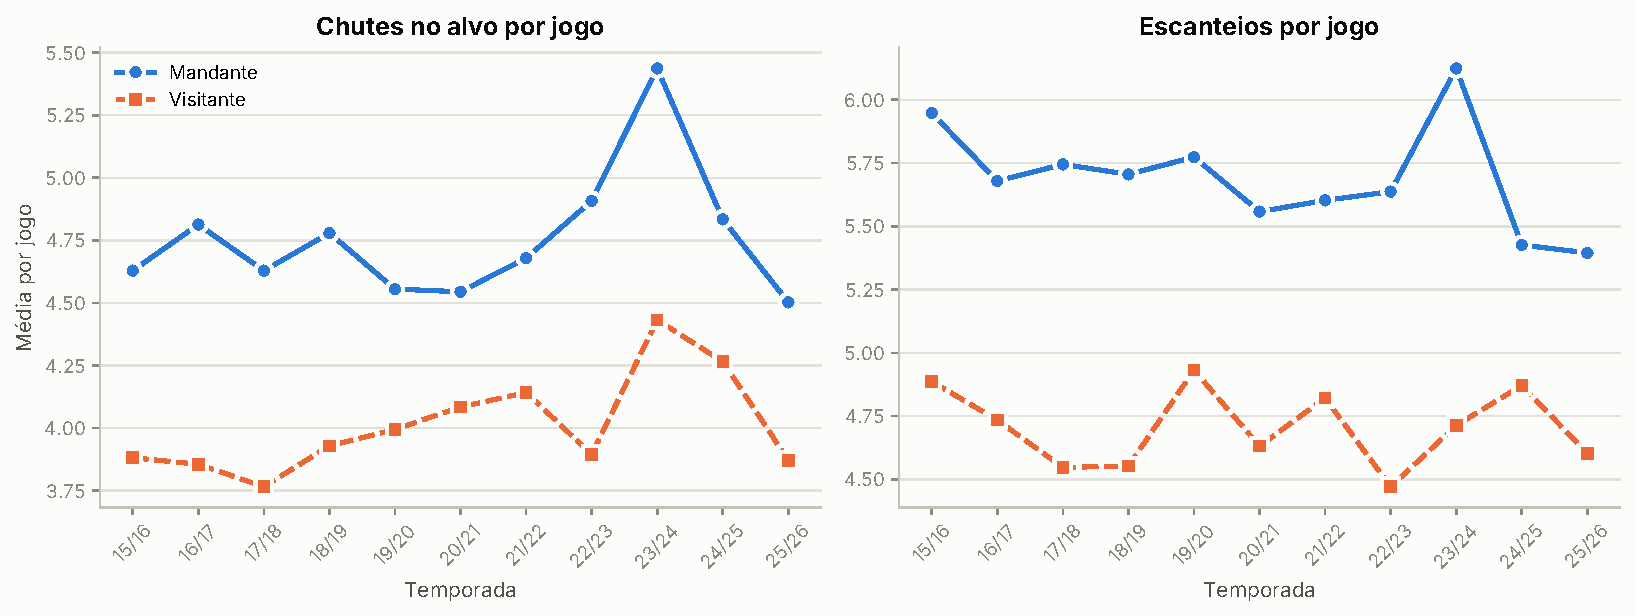
\includegraphics[width=\textwidth]{./figuras/volume_ofensivo.pdf}
  \fonte{Autoria própria (2026)}
\end{figure}

A coluna de cartões amarelos merece destaque. Em todas as temporadas o mandante
recebe menos cartões que o visitante, com diferencial que varia entre $-0{,}02$
e $-0{,}42$. A exceção é justamente 2020/21, temporada em que o diferencial
aproxima-se de zero ($-0{,}024$). Esse comportamento é retomado na
Seção~\ref{sec:res-publico}.

Cabe uma ressalva metodológica quanto à leitura de tendência. O diferencial bruto
de pontos de uma temporada depende não apenas da magnitude do Fator Casa, mas
também da distribuição de força entre os elencos daquele ano e do calendário
efetivamente sorteado. A Seção~\ref{sec:res-modelo} retoma essa questão com uma
métrica que controla por esses fatores.

\section{O Papel do Público}\label{sec:res-publico}

A literatura trata o período de portões fechados como um experimento natural
sobre o papel da torcida. A Tabela~\ref{tab:publico} apresenta o diferencial de
desempenho segundo o regime de público, classificado por data da partida
conforme descrito na Seção~\ref{sec:regime-publico}.

\begin{table}[htb]
  \centering
  \caption{Vantagem do mandante por regime de público.}
  \label{tab:publico}
  \resizebox{\textwidth}{!}{% Gerado por scripts/gerar_tabelas_latex.py --- não editar à mão.
\begin{tabular}{lrrrrrr}
  \toprule
  Cenário & Jogos & Pts casa & Pts fora & $\Delta$ pts & $\Delta$ gols & $\Delta$ amarelos \\
  \midrule
  2019/20 (sem público) & 92 & 1,620 & 1,163 & +0,457 & +0,370 & +0,033 \\
  2019/20 (com público) & 288 & 1,594 & 1,156 & +0,438 & +0,292 & $-$0,247 \\
  demais temporadas (com público) & 3420 & 1,587 & 1,175 & +0,411 & +0,302 & $-$0,215 \\
  2020/21 (público limitado) & 53 & 1,509 & 1,283 & +0,226 & +0,132 & $-$0,377 \\
  2020/21 (sem público) & 327 & 1,330 & 1,450 & $-$0,119 & $-$0,009 & +0,034 \\
  \bottomrule
\end{tabular}
}
  \fonte{Autoria própria (2026)}
\end{table}

\begin{figure}[htb]
  \centering
  \caption{Vantagem do mandante por regime de público.}
  \label{fig:publico}
  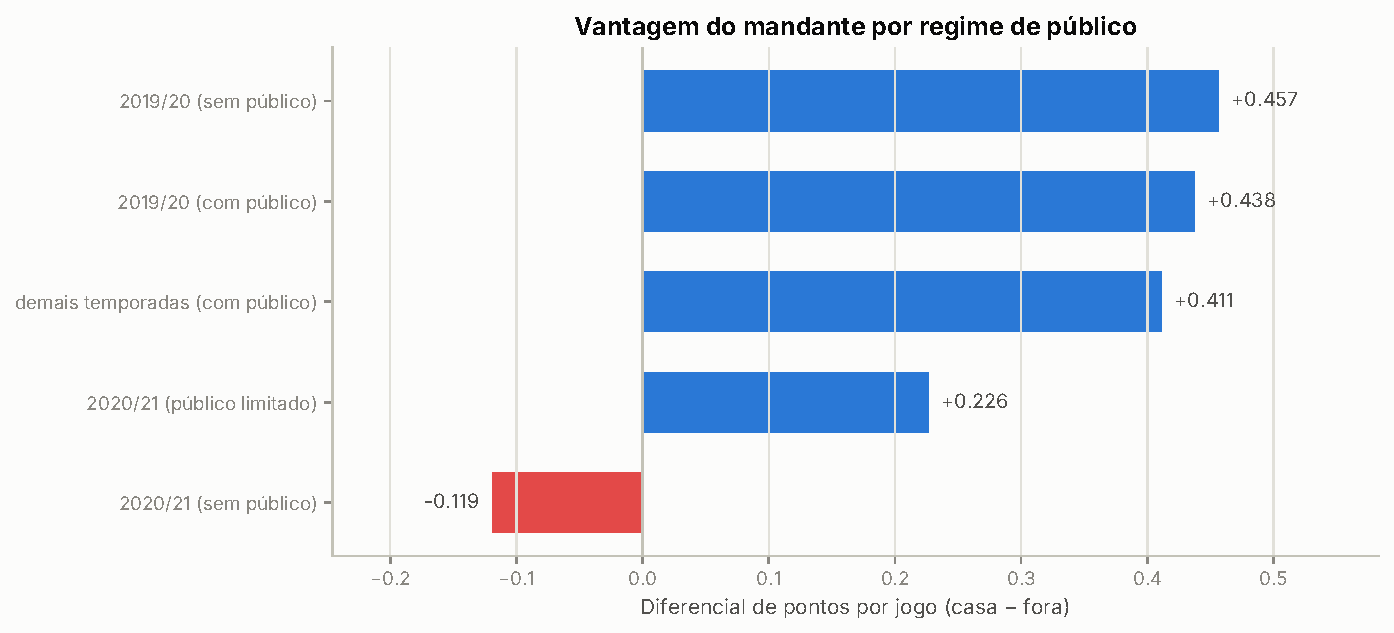
\includegraphics[width=0.95\textwidth]{./figuras/contraste_publico.pdf}
  \fonte{Autoria própria (2026)}
\end{figure}

O contraste decisivo encontra-se nas duas primeiras linhas da tabela. Dentro da
temporada 2019/20 — mesmos elencos, mesmo calendário e mesmo regulamento — as
92 partidas disputadas sem público apresentaram diferencial de $+0{,}457$ ponto,
contra $+0{,}438$ nas 288 partidas com público. A vantagem do mandante não
diminuiu com a ausência de torcida; se algo, foi marginalmente superior. A
diferença não é estatisticamente significativa (Tabela~\ref{tab:testes},
$p = 0{,}952$).

A inversão do Fator Casa manifesta-se exclusivamente em 2020/21, temporada na
qual o diferencial atinge $-0{,}119$ ponto. Essa constatação é relevante porque
2020/21 diferiu das temporadas anteriores em mais aspectos do que a ausência de
público: houve encurtamento da pré-temporada, congestionamento de calendário e
ampliação do número de substituições permitidas. Atribuir a queda
especificamente à ausência de torcida requer supor que nenhum desses fatores
contribuiu, suposição que o contraste de 2019/20 não corrobora.

\subsection{A Separação entre os Mecanismos}\label{sec:res-arbitragem}

A coluna de cartões amarelos da Tabela~\ref{tab:publico} permite uma distinção
que o diferencial de pontos, isoladamente, não permitiria.

Nas partidas com público, o mandante recebe sistematicamente menos cartões
amarelos que o visitante: $-0{,}247$ em 2019/20 e $-0{,}215$ nas demais
temporadas. Nas partidas sem público, essa vantagem desaparece, assumindo
valores praticamente nulos: $+0{,}033$ em 2019/20 e $+0{,}034$ em 2020/21.

O aspecto decisivo é que o desaparecimento ocorre \textbf{já em 2019/20}, mesma
temporada em que a vantagem em pontos não se alterou. Os dois fenômenos, portanto,
dissociam-se: a presença de torcida parece influenciar o comportamento da
arbitragem, conforme sugerido por~\citeonline{Nevill1999}, mas esse viés não é o
mecanismo que sustenta a vantagem do mandante em pontos. Trata-se de evidência a
favor da hipótese de que a familiaridade com o ambiente e o desgaste logístico
imposto ao visitante respondem por parcela mais relevante do fenômeno do que a
pressão da torcida sobre a arbitragem.

\section{Modelagem do Mando de Campo}\label{sec:res-modelo}

As seções anteriores apoiaram-se em médias condicionais, que não controlam pela
identidade dos adversários enfrentados. Esta seção apresenta os resultados do
modelo de Poisson bivariado descrito na Seção~\ref{sec:met-dixon-coles}.

Ajustado sobre o conjunto completo, o modelo estima um parâmetro de mando de
$\gamma = 0{,}1967$, com intervalo de confiança de 95\% entre 0,1605 e 0,2329.
Em termos interpretáveis, jogar em casa está associado a um acréscimo de
\textbf{21,7\% no número esperado de gols}, já descontada a qualidade do
adversário. O parâmetro de correção estimado é $\rho = -0{,}0388$, negativo
conforme previsto por~\citeonline{DixonColes1997}: o modelo de Poisson
independente subestima a frequência de empates de placar baixo.

As forças estimadas ordenam os clubes de maneira compatível com o desempenho
observado no período, com Manchester City e Liverpool no topo, o que constitui
verificação de consistência do ajuste.

\subsection{Evolução do Parâmetro de Mando}\label{sec:res-gamma-temporal}

A Tabela~\ref{tab:gamma} apresenta o parâmetro ajustado separadamente em cada
temporada, com os respectivos intervalos de confiança.

\begin{table}[htb]
  \centering
  \caption{Parâmetro de mando de campo ajustado, por temporada.}
  \label{tab:gamma}
  \small
  % Gerado por scripts/gerar_tabelas_latex.py --- não editar à mão.
\begin{tabular}{lrcr}
  \toprule
  Temporada & $\gamma$ & IC 95\% & Acréscimo de gols \\
  \midrule
  15/16 & 0,2107 & [0,088; 0,333] & 23,5\% \\
  16/17 & 0,2860 & [0,165; 0,407] & 33,1\% \\
  17/18 & 0,2944 & [0,171; 0,418] & 34,2\% \\
  18/19 & 0,2246 & [0,104; 0,345] & 25,2\% \\
  19/20 & 0,2311 & [0,109; 0,354] & 26,0\% \\
  20/21 & 0,0071 & [$-$0,115; 0,129] & 0,7\% \\
  21/22 & 0,1479 & [0,028; 0,268] & 15,9\% \\
  22/23 & 0,2913 & [0,171; 0,412] & 33,8\% \\
  23/24 & 0,1967 & [0,085; 0,308] & 21,7\% \\
  24/25 & 0,0627 & [$-$0,055; 0,180] & 6,5\% \\
  25/26 & 0,2145 & [0,093; 0,336] & 23,9\% \\
  \bottomrule
\end{tabular}

  \fonte{Autoria própria (2026)}
\end{table}

\begin{figure}[htb]
  \centering
  \caption{Parâmetro de mando ajustado por força do adversário, com IC de 95\%.}
  \label{fig:gamma}
  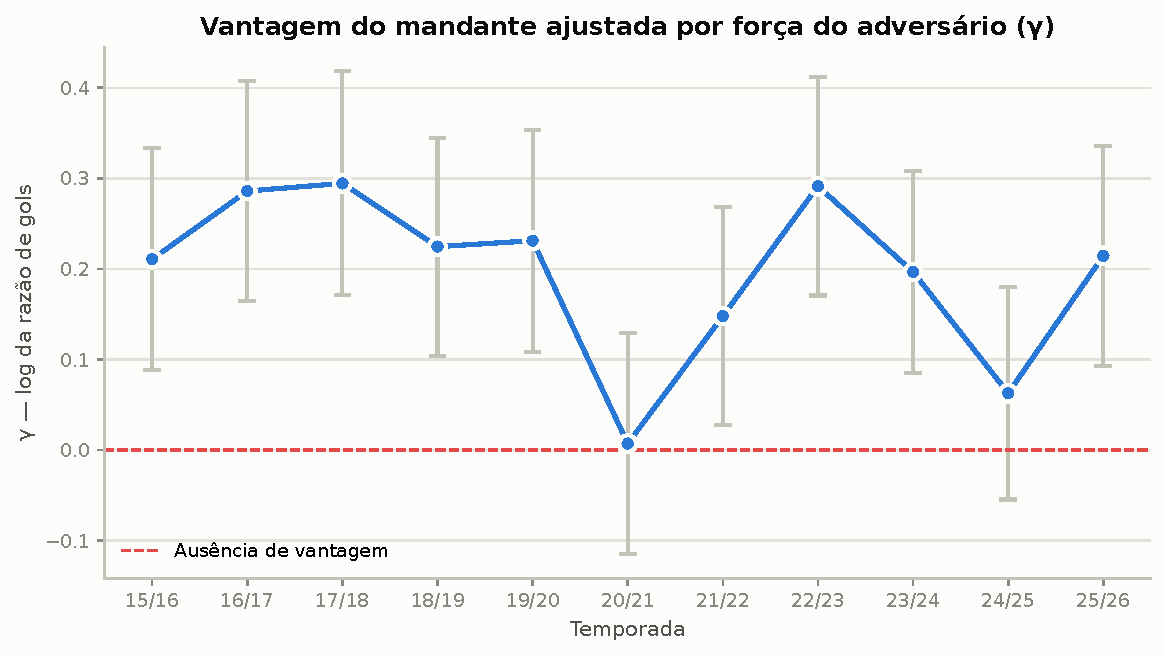
\includegraphics[width=0.95\textwidth]{./figuras/mando_ajustado_por_temporada.pdf}
  \fonte{Autoria própria (2026)}
\end{figure}

Duas temporadas apresentam intervalo de confiança que contém o zero, isto é,
nas quais não se pode rejeitar a hipótese de ausência de vantagem do mandante:
2020/21, já discutida, e \textbf{2024/25}, com $\gamma = 0{,}0627$ e intervalo
entre $-0{,}0547$ e $0{,}1801$. O segundo caso não guarda relação com a pandemia
e não se destacava com a mesma nitidez no diferencial bruto de pontos.

A disponibilidade dos intervalos de confiança impõe cautela à leitura de
tendência. Os intervalos de quase todas as temporadas se sobrepõem, e a
temporada 2022/23 ($\gamma = 0{,}2913$) situa-se no mesmo patamar de 2016/17 e
2017/18. O padrão compatível com os dados é o de \textbf{variabilidade elevada em
torno de um patamar estável, com dois vales}, e não o de uma tendência
monotônica de queda.

\subsection{Efeito do Público Controlado por Adversário}\label{sec:res-gamma-publico}

O contraste descritivo da Seção~\ref{sec:res-publico} não controla pela força
das equipes envolvidas, o que importa porque as partidas sem público de 2019/20
correspondem às rodadas finais, com distribuição de confrontos distinta da
temporada completa. A Tabela~\ref{tab:delta} apresenta a estimativa do
deslocamento~$\delta$ do parâmetro de mando associado à ausência de público.

\begin{table}[htb]
  \centering
  \caption{Efeito da ausência de público sobre o parâmetro de mando.}
  \label{tab:delta}
  \resizebox{\textwidth}{!}{% Gerado por scripts/gerar_tabelas_latex.py --- não editar à mão.
\begin{tabular}{lrrccr}
  \toprule
  Recorte & $\gamma$ & $\delta$ & IC 95\% & $p$ & $n$ sem / com \\
  \midrule
  2019/20 (intratemporada) & 0,2213 & +0,0402 & [$-$0,150; 0,231] & 0,680 & 92 / 288 \\
  recorte completo (19/20 + 20/21) & 0,2094 & $-$0,1225 & [$-$0,209; $-$0,036] & 0,006 & 419 / 3708 \\
  \bottomrule
\end{tabular}
}
  \fonte{Autoria própria (2026)}
\end{table}

Dentro da temporada 2019/20, a estimativa é $\delta = +0{,}0402$, com intervalo
entre $-0{,}1505$ e $+0{,}2308$ e $p = 0{,}680$: não há efeito detectável.
Considerando o conjunto das partidas sem público, a estimativa torna-se
$\delta = -0{,}1225$, com intervalo entre $-0{,}2095$ e $-0{,}0355$ e
$p = 0{,}006$, portanto significativa.

A conciliação entre os dois resultados é direta: 327 das 419 partidas sem
público pertencem à temporada 2020/21. O efeito agregado é determinado por essa
temporada. Convém explicitar o alcance dessa conclusão: o intervalo obtido para
2019/20 ainda contém o valor estimado no agregado, de modo que os dados
\textbf{não excluem} um efeito daquela magnitude. Tampouco é possível construir
o contraste dentro de 2020/21, pois nenhuma partida daquela temporada foi
disputada com público pleno segundo a classificação adotada.

O que se pode afirmar com segurança é que a vantagem do mandante reduziu-se
praticamente a zero em 2020/21, e que a atribuição dessa redução especificamente
à ausência de torcida é uma inferência que o contraste intratemporada disponível
não corrobora. Essa conclusão diverge de parte da literatura que tratou o
episódio como isolamento limpo da variável público e, à luz da dissociação
apresentada na Seção~\ref{sec:res-arbitragem}, sugere que o papel da torcida
opera preferencialmente sobre o comportamento da arbitragem.

\section{Modelagem Preditiva}\label{sec:res-preditivo}

A Tabela~\ref{tab:preditivo} apresenta o desempenho dos modelos preditivos sob
validação temporal, agregado sobre as oito temporadas de teste, totalizando
3.040 partidas.

\begin{table}[htb]
  \centering
  \caption{Desempenho preditivo sob validação temporal.}
  \label{tab:preditivo}
  \small
  % Gerado por scripts/gerar_tabelas_latex.py --- não editar à mão.
\begin{tabular}{lrrrr}
  \toprule
  Modelo & \textit{Log-loss} & Brier & Acurácia & $n$ \\
  \midrule
  Dixon-Coles & 0,9762 & 0,5785 & 53,6\% & 3040 \\
  Regressão logística & 0,9880 & 0,5834 & 53,6\% & 3040 \\
  Frequência base & 1,0669 & 0,6457 & 43,9\% & 3040 \\
  Sempre o mandante & 1,0747 & 0,6500 & 43,9\% & 3040 \\
  \textit{Gradient boosting} & 1,0807 & 0,6257 & 50,7\% & 3040 \\
  \bottomrule
\end{tabular}

  \fonte{Autoria própria (2026)}
\end{table}

\begin{figure}[htb]
  \centering
  \caption{Desempenho preditivo dos modelos avaliados.}
  \label{fig:preditivo}
  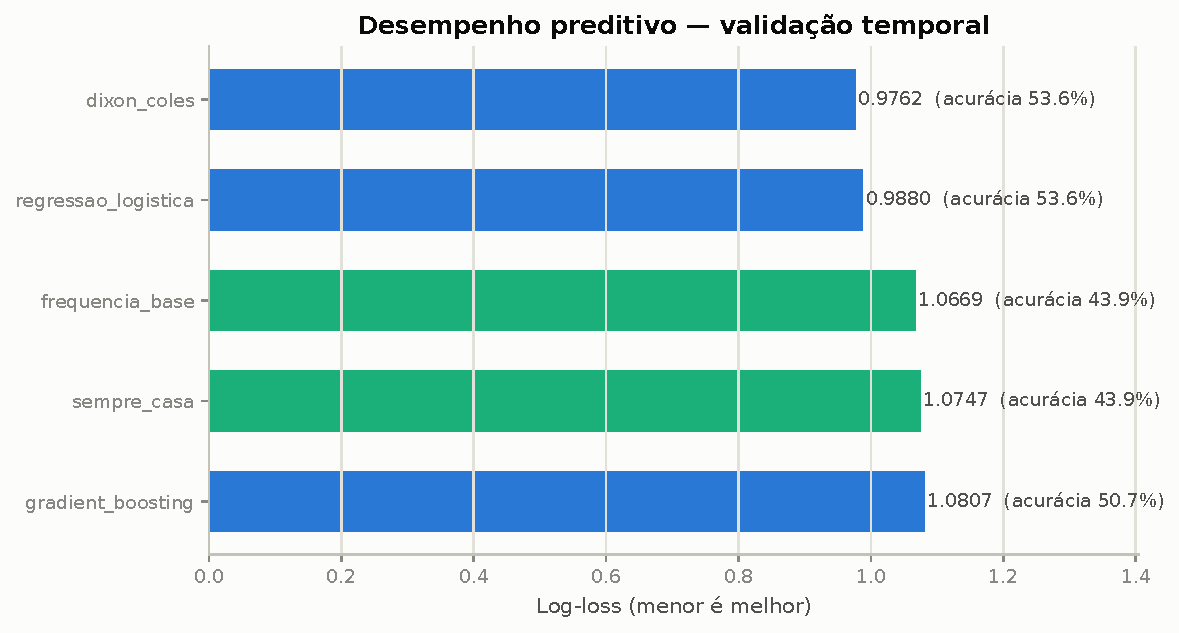
\includegraphics[width=0.9\textwidth]{./figuras/preditivo_desempenho.pdf}
  \fonte{Autoria própria (2026)}
\end{figure}

Três leituras merecem destaque.

A primeira é que \textbf{o modelo estatístico superou os modelos de aprendizado
de máquina}. O modelo de Poisson bivariado obteve o menor \textit{log-loss}
(0,9762) e o menor escore de Brier (0,5785), liderando em seis das oito
temporadas avaliadas, com a regressão logística em posição próxima (0,9880).
Esse resultado é coerente com a natureza do problema: o modelo de Poisson
incorpora a estrutura geradora dos dados — gols são contagens, cada clube possui
capacidades distintas de ataque e defesa, e o mando desloca a média esperada —
em vez de precisar inferi-la a partir de um conjunto limitado de variáveis
explicativas.

A segunda é que \textbf{o modelo de \textit{gradient boosting} obteve desempenho
inferior ao da frequência base} segundo o \textit{log-loss} (1,0807 contra
1,0669), apesar de apresentar acurácia substancialmente superior (50,66\% contra
43,95\%). Essa combinação é característica de um modelo mal calibrado e
constitui a justificativa empírica para a escolha de métricas discutida na
Seção~\ref{sec:avaliacao}.

A terceira é que todos os modelos superam a heurística de prever sempre a
vitória do mandante, que atinge 43,95\% de acurácia, contra 53,59\% do modelo de
Poisson. O ganho é real, porém modesto, o que evidencia o teto de
previsibilidade característico da modalidade.

\subsection{Análise de Calibração}\label{sec:res-calibracao}

A Figura~\ref{fig:calibracao} compara, em faixas de probabilidade prevista, a
frequência efetivamente observada de vitórias do mandante.

\begin{figure}[htb]
  \centering
  \caption{Curvas de calibração para a previsão de vitória do mandante.}
  \label{fig:calibracao}
  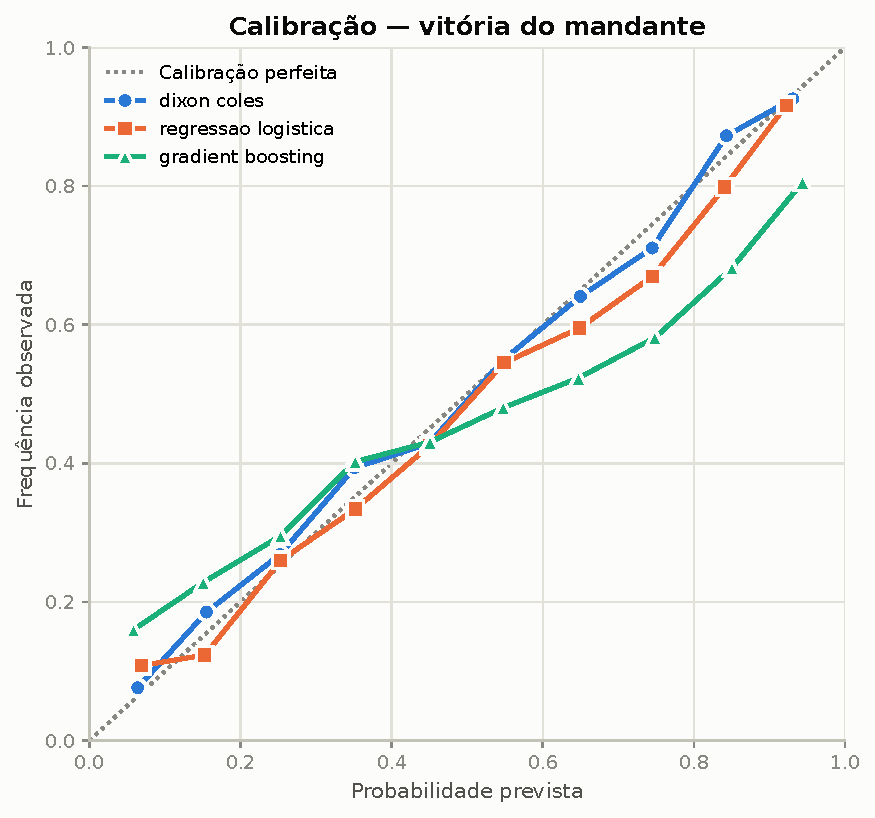
\includegraphics[width=0.72\textwidth]{./figuras/preditivo_calibracao.pdf}
  \fonte{Autoria própria (2026)}
\end{figure}

O modelo de Poisson e a regressão logística situam-se próximos à diagonal, o que
indica boa calibração. O modelo de \textit{gradient boosting}, por sua vez,
apresenta desvio sistemático em ambos os extremos: nas partidas às quais atribui
94\% de probabilidade de vitória do mandante, a frequência observada é de 81\%;
naquelas às quais atribui 6\%, o evento ocorre em 16\% dos casos.

O comportamento é internamente consistente com as métricas da
Tabela~\ref{tab:preditivo}. Ao deslocar as probabilidades em direção aos
extremos, o modelo acerta mais frequentemente a classe mais provável — o que
eleva a acurácia — e simultaneamente incorre em penalizações severas do
\textit{log-loss} nas previsões confiantes e incorretas. Esse resultado ilustra,
de forma concreta, por que a acurácia é insuficiente como critério único de
avaliação em problemas probabilísticos.

Observa-se ainda que todos os modelos apresentam desempenho pior na temporada
2020/21. Na ausência da vantagem do mandante, o preditor mais informativo do
problema perde força, e a previsão torna-se mais difícil para todos os métodos
avaliados — resultado que conecta a etapa preditiva à análise do Fator Casa
conduzida nas seções anteriores.

\section{Estudo de Caso: Mudança de Estádio}\label{sec:resultados-estadios}

A arquitetura e a atmosfera do estádio constituem variável qualitativa
frequentemente associada ao Fator Casa. Esta seção examina o desempenho de
clubes que mudaram de sede durante o período analisado.

A análise exige recorte estendido, iniciado em 2009/10, pois o recorte principal
não oferece linha de base anterior às mudanças. Conforme a
Seção~\ref{sec:quebras}, métricas de finalização não são comparáveis através da
fronteira de 2013/14 e, por essa razão, foram omitidas da
Tabela~\ref{tab:estadios}. O Brentford, que disputou a \textit{Premier League}
apenas a partir de 2021/22, já em sua nova sede, não possui período anterior e
foi excluído da análise.

\begin{table}[htb]
  \centering
  \caption{Desempenho antes e depois da mudança de estádio.}
  \label{tab:estadios}
  \resizebox{\textwidth}{!}{% Gerado por scripts/gerar_tabelas_latex.py --- não editar à mão.
\begin{tabular}{lllrrrr}
  \toprule
  Clube & Período & Estádio & Jogos casa & Pts casa & Pts fora & $\Delta$ pts \\
  \midrule
  West Ham & Antes & Boleyn Ground (Upton Park) & 114 & 1,474 & 0,826 & +0,648 \\
  West Ham & Depois & London Stadium & 190 & 1,421 & 1,074 & +0,347 \\
  Tottenham & Antes & White Hart Lane / Wembley & 185 & 2,103 & 1,654 & +0,448 \\
  Tottenham & Depois & Tottenham Hotspur Stadium & 138 & 1,696 & 1,281 & +0,414 \\
  \bottomrule
\end{tabular}
}
  \fonte{Autoria própria (2026)}
\end{table}

O West Ham United apresentou redução expressiva: de $+0{,}648$ ponto por partida
no Boleyn Ground para $+0{,}347$ no London Stadium, aproximadamente metade da
vantagem anterior. O Tottenham Hotspur, por sua vez, manteve desempenho
praticamente inalterado, passando de $+0{,}448$ para $+0{,}414$.

O resultado é sugestivo e compatível com a hipótese de que arenas modernas, de
maior capacidade e com afastamento entre arquibancada e campo, diluiriam a
pressão exercida sobre o visitante. Deve, contudo, ser interpretado como
\textbf{estudo de caso exploratório}. São apenas dois clubes, e os períodos
posteriores às mudanças coincidem com alterações de elenco, de comissão técnica e
de patamar competitivo que não foram controladas. A evidência é insuficiente para
sustentar afirmação causal.
